\chapter{Benchmark-II}

\section{The Task}
The objective of the program is simple. The function takes an input array, A, and multiplies it by a constant here \textbf{2} to create a new array. In this operation, array multiplication is performed on both the CPU and the GPU, and reports the process times taken on the two. These two numbers are measured for a range of process size (total number of operations required for the process).\\

\section{Code Walktrough}
Code Walkthrough mentioned in file codewalkthrough.

\section{Results}
The program depicits the capabilities of CPU and GPU indivudially. Elements in array v/s time taken in CPU has a constant positive slope whereas the slope for the same graph plotted is zero. No matter how many elements are in array, the time taken by GPU remains constant (with very slight variation). There are few points where the graph shoots up for both CPU and GPU.

\subsection{Output}
The output of the program in which the array is multiplied with a constant \textbf{'2'} have been mentioned in the following files :\\\\
\begin{enumerate}
\item gpuresult for GPU Result\\
\item cpuresult for CPU Result\\
\end{enumerate}
\subsection{Plots}
\vspace{1cm}
\textbf{CPU vs GPU}\\\\
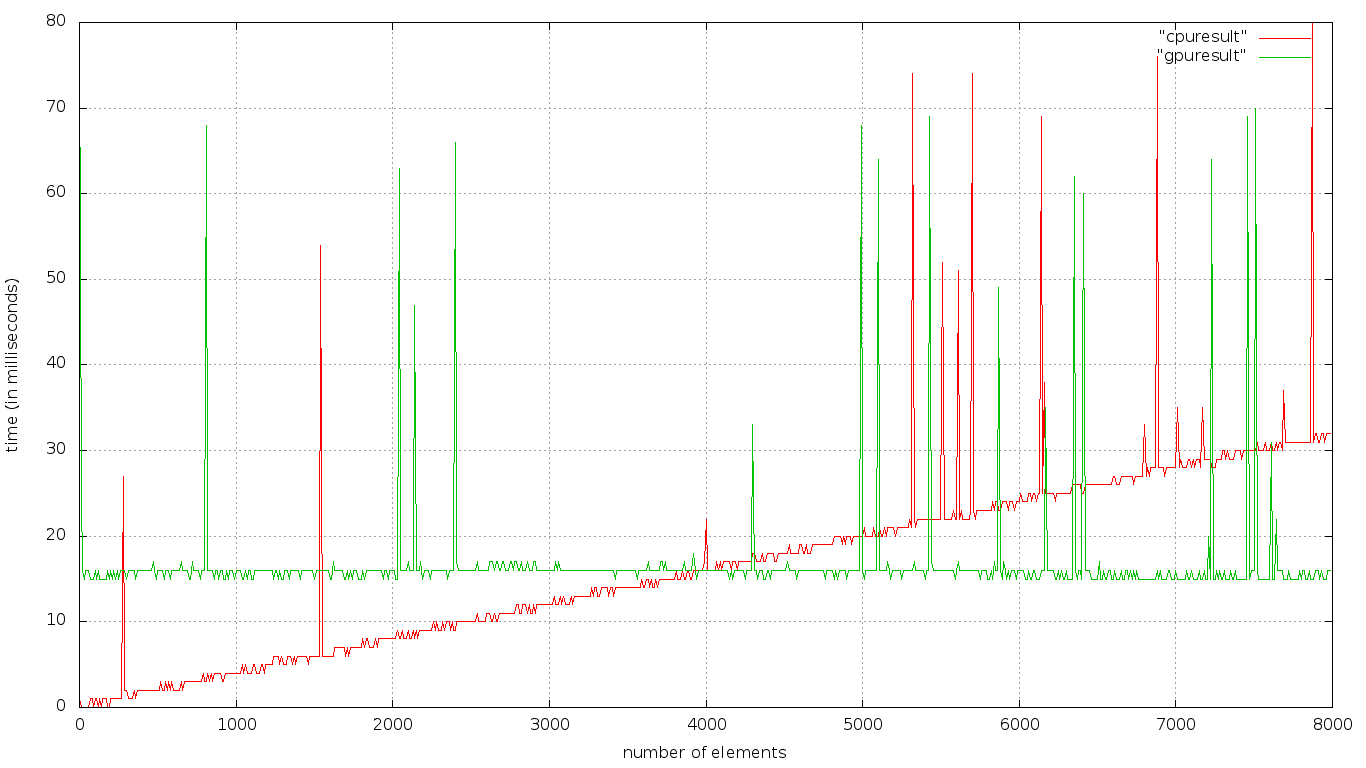
\includegraphics [width=1.2\textwidth]{plot1.png}

\section{Inferences}
\begin{enumerate}
\item When this code is run, you will find that the CPU is faster than the GPU for an array of 3,900 elements. If you increase the size to 3,900 to about 4,000 elements in the array, the two will essentially tie. Above 4,000 elements in the array, and the GPU will win. 
\item The threads should be running in groups of at least 32 (since the kernel issues commands equal to the warp size [32 in our case]) for best performance, with total number of threads numbering in the thousands. Branches in the program code do not impact performance significantly, provided that each of 32 threads takes the same execution path; the SIMD execution model becomes a significant limitation for any inherently divergent task.
\item The overhead in creating threads on GPU kernel remains same, it does not depends on the number of elements. 
\end{enumerate}

